\documentclass[english]{exam}

\setlength {\marginparwidth }{2cm} 
\usepackage{todonotes}

\usepackage[perpage,para,symbol]{footmisc}

\hyphenpenalty=15000 
\tolerance=1000

\usepackage{tikz}
\usetikzlibrary{arrows,decorations.pathmorphing,backgrounds,fit,positioning,calc,shapes}
\usepackage{pgfmath}
\usepackage{rotating}
\usepackage{array}	
\usepackage{graphicx}
\usepackage{float}	
\usepackage{mdwlist}
\usepackage{setspace}
\usepackage{listings}
\usepackage{bytefield}
\usepackage{tabularx}
\usepackage{multirow}	       
\usepackage{caption}
\usepackage{xcolor}
\usepackage{amssymb}
\captionsetup[table]{skip=10pt}

\usepackage{url}
\usepackage{hyperref}
\usepackage[all]{hypcap}	
\usepackage{titlesec}
\setcounter{secnumdepth}{4}
\titleformat{\paragraph}
{\normalfont\normalsize\bfseries}{\theparagraph}{1em}{}
\titlespacing*{\paragraph}
{0pt}{3.25ex plus 1ex minus .2ex}{1.5ex plus .2ex}

\definecolor{mGreen}{rgb}{0,0.6,0}
\definecolor{darkblue}{rgb}{0.1,0.1,0.5}
\definecolor{mGray}{rgb}{0.5,0.5,0.5}
\definecolor{mPurple}{rgb}{0.58,0,0.82}
\definecolor{backgroundColour}{rgb}{0.95,0.95,0.92}

\hypersetup{colorlinks,breaklinks,
            linkcolor=darkblue,urlcolor=darkblue,
            anchorcolor=darkblue,citecolor=darkblue}


\lstdefinestyle{CStyle}{
    backgroundcolor=\color{backgroundColour},   
    commentstyle=\color{mGreen},
    keywordstyle=\color{magenta},
    numberstyle=\tiny\color{mGray},
    stringstyle=\color{mPurple},
    basicstyle=\footnotesize,
    breakatwhitespace=false,         
    breaklines=true,                 
    captionpos=b,                    
    keepspaces=true,                 
    numbers=left,                    
    numbersep=5pt,                  
    showspaces=false,                
    showstringspaces=false,
    showtabs=false,                  
    tabsize=2,
    language=C
}

\NewDocumentCommand{\codeword}{v}{%
  \texttt{
  \colorbox{backgroundColour}{\textcolor{magenta}{#1}}}%
}


\PassOptionsToPackage{USenglish,english}{babel} 
\usepackage{csquotes}
\usepackage{tabto}
\usepackage[USenglish,english]{babel}
\usepackage[acronym, section=section, nonumberlist, nomain, nopostdot]{glossaries}
\makeglossaries
 
\makeglossaries
\newcommand{\colorbitbox}[3]{%
	\rlap{\bitbox{#2}{\color{#1}\rule{\width}{\height}}}%
	\bitbox{#2}{#3}}


\begin{document}

\title{Assignment IV:\\ OpenCL and OpenACC}
\author{Amirhossein Namazi, Calin Capitanu}

\maketitle
\begin{center}
  \url{https://github.com/capitanu/DD2360} \\
\end{center}

\chapter{Exercise 1}
\section*{Hello World!}

The first part of the assignment was to extend the template to have a working OpenCL application. Initially, we had to run the actual OpenCL app within a string declared at the top of the C code. This part of the program is just suppossed to print ``Hello World'' together with the ID of the work item. The ID is retrieved with the command \codeword{get_global_id()}. \\
Next up, we had to actually create the program from the string and build it, while also checking for possible errors. After we do this and also create the kernel, while specifying the number of work items and the workgroup size, we enqueue the kernel to be run and wait for it to be finished.
\\\\
In the first part of the assignment where we only had 1 dimension to the number of workitems, everything was straight-forward, however in the second part we had to create a 2 dimensional array and later a 3 dimensional array. The changes for these were only regarding the number of workitems and the workgroup size, such that these, instead of being integers, would be arrays of sizes and finally specyinf the size in the enqueue command as such:\\
\codeword{clEnqueueNDRangeKernel(cmd_queue, kernel, 3, NULL, &n_workitem, &workgroup_size, 0, NULL, NULL);}\\\\
Finally, after doing this for the 2D and then 3D arrays, we also had to figure out how to print the index of each workitem. In OpenCL this is made a lot easier by the availability of two different commands, depending on the point of reference of the index: either global or local, with the commands \codeword{get_global_id()} and \codeword{get_local_id()}. These two come together with the command \codeword{get_group_id()} in order to be able to also compute the global id from the local id and the group id. It is also pretty convinient that we can query the index on different axis.

\clearpage
\chapter{Exercise 2}
\section*{Performing SAXPY using OpenCL}

This whole exercise was pretty much similar to the CUDA SAXPY exercise since we already had the boiler-plate code of setting up OpenCL from the previous assignment (and one must be crazy re-writing it), and then a lot of code from Assignment 2 in SAXPY could have still be used in this assignment.
\\\\
In order to have the number of workitems match the workgroup size, we just had to add to it the difference until it would be a multiple of \codeword{workgroup_size}. This was a pretty simple mathematical trick that did the job: 
\codeword{size_t n_workitem = size + (workgroup_size - size % workgroup_size);}.
Where \codeword{size} is the length of the array itself.
\\\\

Since timing this would have not been such an issue (because we could easily reuse the previous functions from Assignment 2), we decided to do so, and finally to plot the graphs and insert them into this report:

  \begin{center}
    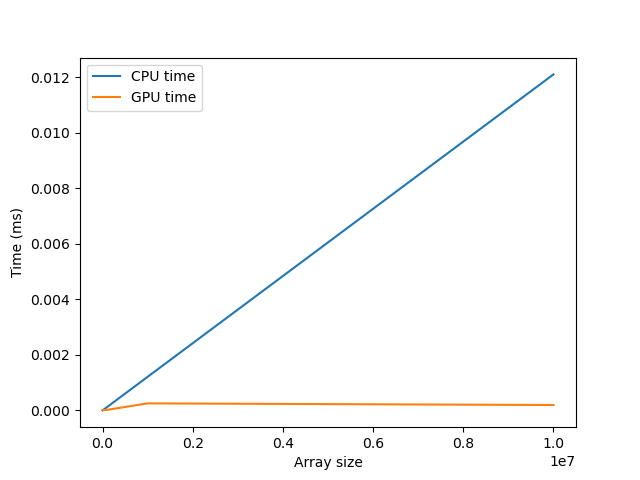
\includegraphics[scale=0.65]{plot1.png}
  \end{center}

\clearpage
\chapter{Exercise 3}
\section*{Performing SAXPY using OpenACC}

It is surprising to us to observe such a low performance of the OpenACC program. Just to make sure we got this right, we need to specify that we ran all the commands as suggested in the lecture, using the \codeword{-acc} flag while running \codeword{pgcc}. The results we got were far worse than even the CPU performance we got before. We have plotted below all three of the results for a better understanding:

  \begin{center}
    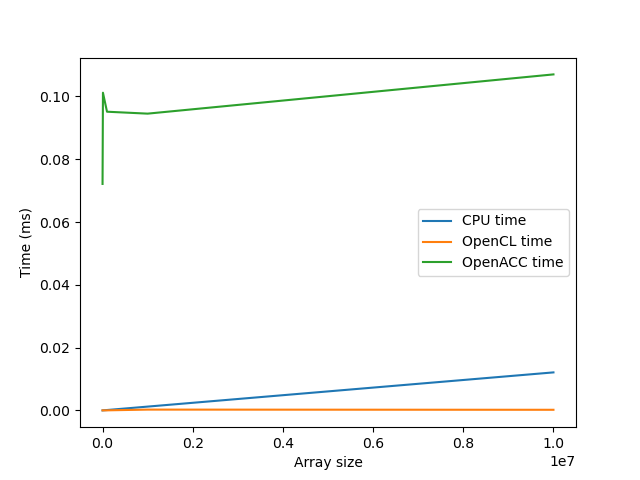
\includegraphics[scale=0.65]{plot2.png}
  \end{center}

  However, an interesting thing to notice is the fact that once we increase the array size linearly, with increments of x10, we observe that the time taken to perform these calculations does not increase linearly, which is the case for the CPU variant. With some enormous amount of elements in the list, we might get better performance with OpenACC, however it does not seem worth as it is right now.

\clearpage
\chapter{Exercise 4}
\section*{Discuss, Reflect, Contrast}

The first point that we want to touch is the usability of both OpenCL and OpenACC. The latter, OpenACC is such an easy tool to use that one must not know how to write anything else than basic C, while then adding some directives. The basic SAXPY CPU version only needed 1 extra line added, which is amazing and I would assume that it would make development way easier and less expensive, since developers that are specialized on something niche are usually more expensive. \\\\
On the other hand, OpenCL seems to be a lot harder to write. While it is not hard to understand, there are a lot of failing points where one can get stuck for a long time. For example, in my case, OpenCL could not find any platforms, which took way too long to figure out and to fix, only to find out later that cuda has already packed a specific tool-kit, but it also has to be of the matching version with the CUDA driver - all plus the linux problems that cuda comes with, which are well known. \\
In OpenCL, there is a lot of boiler plate code that could be omitted, however, we also see the amount of customization and how specific one could be by having to run all of the commands to specify a platform and such. \\
Finally, on OpenCL, it is really inconvenient to write code inside of strings. That is, most text editors don't expect that, thus the formatting for this becomes really messy and unreadable.
\\\\
To compare these to CUDA, for me it seems like CUDA is placed somewhere in the middle in terms of difficulty, since we considered OpenACC to be too easy to write, while in CUDA you also have to specify some particularities.
\\\\
When talking about performance, it is easiest to take an example and examine it:
  \begin{center}
    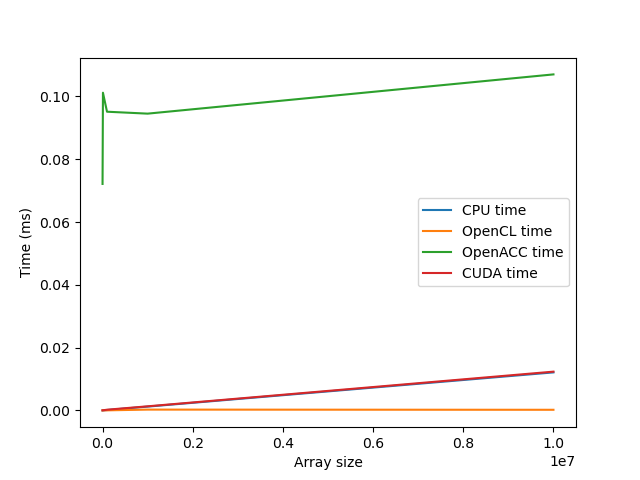
\includegraphics[scale=0.6]{plot3.png}
  \end{center}
We can see in the image above that the OpenACC implementation is by far the worst, while the OpenCL is the best performer. Since the graph is scaled in order to fit the huge gaps in between, CPU and GPU CUDA times seem to be the same, however for the examples, the CUDA implementation is slighlty worse, maybe by a fraction of $1\%$.
\\\\
To conlcude, our guess is that CUDA is still one of the most used environments for GPU development just because of the size of the company and the market share, however, with the new AMD GPU series, this things might change. 

\clearpage
\chapter{Bonus Exercise}
\section*{OpenCL Particles Simulations}

The results after running this experiment were sort of expected. The CPU time had overall way worse time than the GPU version of the same program, even though we consider the copying time for the data in the GPU. The differences are in the range of x100 apart. Besides these, the really interesting part of our result is the difference in the results. However, it is obvious by printing the positions at the end that nothing in the program itself is wrong, which is a good thing to know, but the final difference in the position of the particles between CPU and GPU grows exponentially with the number of iterations (which could somehow make sense).
\\\\
  \begin{center}
    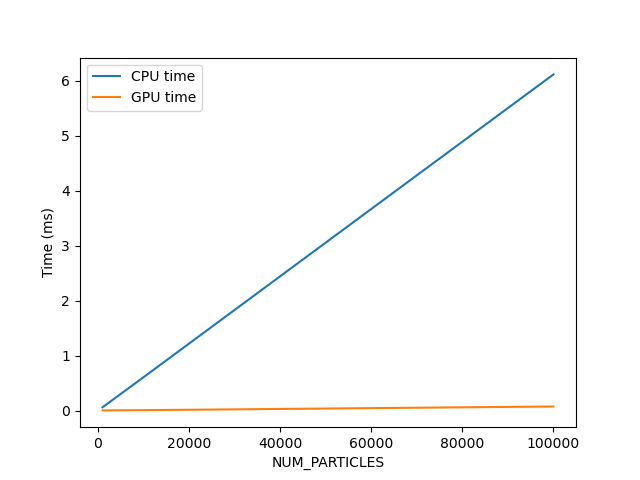
\includegraphics[scale=0.6]{plot4.png}
  \end{center}
\noindent
Here are some results from the CPU version of the program in a table for different number of particles:
\\
\begin{center}
  \begin{tabular}{ |p{4cm}||p{4cm}|p{4cm}|  }
    \hline
    \multicolumn{3}{|c|}{CPU times} \\
    \hline
    Time (seconds)& NUM\_PARTICLES& NUM\_ITERATIONS\\
    \hline
    0.061030& 1000& 10000\\
    0.608230& 10000& 10000\\
    6.115252& 100000& 10000\\
    \hline
  \end{tabular}
\end{center}

\noindent
It is pretty obvious that the time increases linearly with the number of particles in the CPU version, which is also something expected since this is a sequential work.\\
The results seem to be way better for the GPU version, which we have included in the table below for a number of different particles and different block sizes.\\

\begin{center}
    \begin{tabular}{ |p{3cm}||p{3cm}|p{3cm}|p{3cm}|  }
    \hline
    \multicolumn{4}{|c|}{GPU times} \\
    \hline
    Time (seconds)& NUM\_PARTICLES& NUM\_ITERATIONS&BLOCK SIZE\\
    \hline
    0.000843& 1000& 10000& 16\\
    0.000848& 1000& 10000& 32\\
    0.000897& 1000& 10000& 64\\
    0.000943& 1000& 10000& 128\\
    0.004488& 1000& 10000& 256\\
    0.003809& 10000& 100000& 16\\
    0.004856& 10000& 100000& 32\\
    0.003559& 10000& 100000& 64\\
    0.004303& 10000& 100000& 128\\
    0.008764& 10000& 100000& 256\\
    0.053141& 100000& 100000& 16\\
    0.066645& 100000& 100000& 32\\
    0.065236& 100000& 100000& 64\\
    0.065573& 100000& 100000& 128\\
    0.075314& 100000& 100000& 256\\
    \hline
  \end{tabular}
\end{center}

On average, the better results seem to be with a smaller block size on the GPU, however, any of the results displayed in the above table are obviously better than the CPU version of the same program.
\\\\
In order to better visualize the results, I have created a plot with all of them.
\\
\begin{center}
  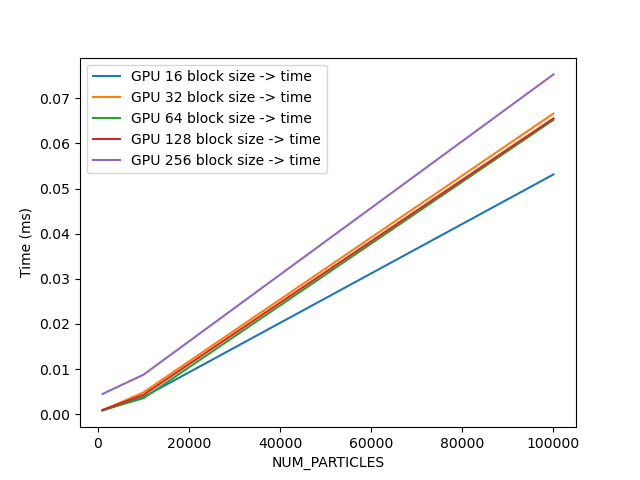
\includegraphics[scale=0.6]{plot5.png}
\end{center}
\noindent
Were I to include the CPU times in the same graph, it would have scaled the whole thing to where the difference would not be observable, thus it has been left out for this experiment. The device on which this experiment has been run on is an NVIDIA RTX 3080 that is overclocked. It seems, by inspecting the graph above, that the smallest block size is the most favorable for this configuration and this specific task. \\
The execution time seems to increase sublinearly, which is really good results for it, comparing it to the CPU version.
\\\\
Finally, for the last question in this assigment, it is pretty obvious to me that the whole execution time of the kernel would drastically increase due to moving of data. We already know that the PCIe lanes have a narrower badnwidth and the transmissions rate are not the greatest (when compared to internal memory). Having one copy per iterations is really costly and inefficient.

\bibliographystyle{myIEEEtran}
\renewcommand{\bibname}{References}
\addcontentsline{toc}{chapter}{References}
\bibliography{references}

\end{document}
